% status: 100
% chapter: TBD

\title{Automated Apache Spark Cluster Deployment on AWS EC2 using Ansible}


\author{Sandeep Khandelwal}
\affiliation{%
  \institution{Indiana University}
  \city{Bloomington} 
  \state{IN} 
  \postcode{47408}
  \country{USA}}
\email{skhande@iu.edu}



% The default list of authors is too long for headers}
\renewcommand{\shortauthors}{Sandeep}


\begin{abstract}

This project is about developing a module for automated deployment of
Apache Spark Cluster on AWS (Amazon Web Services) EC2 (Elastic Compute
Cloud) instances on a single click and performs various data
processing related tasks on Apache Spark Cluster. This project
provides option to terminate the Apache Spark Cluster once data
processing task is completed. This project also does the benchmarking
of deployment, data processing and termination of the instances.

\end{abstract}

\keywords{hid-sp18-511, AWS, EC2, Apache Spark, Apache Hadoop, Ansible}


\maketitle

\section{Introduction}

This module does infrastructure related tasks of provisioning of
AWS~\cite{hid-sp18-511-www-aws} EC2~\cite{hid-sp18-511-www-ec2}
instances, setting up the public/private key pair for secure
connection with EC2~\cite{hid-sp18-511-www-ec2} instance and configure
inbound/outbound traffic rules on provisioned machines to allow
connectivity on various ports. This module also perform Apache
Spark~\cite{hid-sp18-511-www-spark} installation on the provisioned
EC2~\cite{hid-sp18-511-www-ec2} instances using master/worker model
and perform all required configuration. One of the machine will work
as a master node and other machines will work as worker node. User can
do various data processing related tasks once Apache
Spark~\cite{hid-sp18-511-www-spark} Cluster is setup. Apache
Spark~\cite{hid-sp18-511-www-spark} Cluster can be terminated once
data processing related task complete.

The module expose command line options for Apache
Spark~\cite{hid-sp18-511-www-spark} Cluster deployment and termination
of machines once the data processing related task complete. User can
connect to Apache Spark~\cite{hid-sp18-511-www-spark} Cluster and
perform various data related tasks. Benchmarking is done for measuring
the deployment, data processing and termination of the instances.

Ansible~\cite{hid-sp18-511-www-ansible} automation tool is used in
this project to provision EC2~\cite{hid-sp18-511-www-ec2} instances,
deploy Apache Spark~\cite{hid-sp18-511-www-spark} Cluster on
EC2~\cite{hid-sp18-511-www-ec2} instance and terminate
AWS~\cite{hid-sp18-511-www-aws} EC2~\cite{hid-sp18-511-www-ec2}
instances once the data processing related task complete.

\section{Technologies Used}

This section describes the technology used in the project including
AWS~\cite{??} (see Section~\ref{S:aws}), Apache Spark~\cite{??}, and
Ansible~\cite{??}.

\subsection{AWS}\label{S:aws}

AWS~\cite{hid-sp18-511-www-aws} is a secure cloud service provider
that provide various on-demand services.
AWS~\cite{hid-sp18-511-www-aws} provides services in Compute, Storage,
Database, Migration, Networking and Content Delivery, Developer Tools
and many more. These services are easy to setup and can be configured
in few minutes. All the services are on demand service and
AWS~\cite{hid-sp18-511-www-aws} charge only for the duration service
is being used. This is very effective and suitable for both small and
large customers.

The following AWS configuration is used in this project:

\begin{itemize}
	\item \verb|project_name: ec2_spark|
	\item \verb|region: us-west-2|
	\item \verb|env: stg|
\end{itemize}


\subsection{EC2}

EC2~\cite{hid-sp18-511-www-ec2} is AWS secure and resizable compute
service. EC2~\cite{hid-sp18-511-www-ec2} instances can be created on
demand with different configuration of memory, CPU power and hard
disk. EC2~\cite{hid-sp18-511-www-ec2} instances can be added and
terminated at run time based on the load of application. Adding or
terminating EC2~\cite{hid-sp18-511-www-ec2} instances is very easy and
can be done in few minutes.

Two EC2~\cite{hid-sp18-511-www-ec2} instances are created in this
project with following configuration. One of the instance is used for
master node and another one for worker node.

Table~\ref{t:ec2-configuration} provides the
EC2~\cite{hid-sp18-511-www-ec2} configuration details.

\begin{table}[]
	\centering \caption{Configuration}\label{t:ec2-configuration}
  \begin{tabular}{lllll} \textbf{Node}
	& \textbf{AMI} & \textbf{CPUs} & \textbf{RAM}
	& \textbf{Disk}\\ Apache Spark Master & ami-4e79ed361 & 1 & 2
	GB & 8GB\\ Apache Spark Worker & ami-4e79ed361 & 1 & 2 GB & 8GB\\ 
  \end{tabular}
\end{table}

\subsection{Security Group}

A \emp{Security Group} restricts the inbound and outbound traffic for
EC2~\cite{hid-sp18-511-www-ec2} instance.  We can define the allowed
incoming and outgoing traffic using Security Group and assign it to
the instance. Security Group works as firewall and allow only
permitted traffic on EC2~\cite{hid-sp18-511-www-ec2} instance.

We create the security group \verb|ec2_spark_stg_security_group| with the
following inbound and outbound ports open in this project and assign
it to the EC2~\cite{hid-sp18-511-www-ec2} instances created.

\begin{itemize}
	\item \verb|Inbound: 80, 8080, 22, 7178, 8181, 7077, 443|
	\item \verb|Outbound: all|
	
\end{itemize}

\subsection{Key Pair}

Key Pair is used to connect EC2~\cite{hid-sp18-511-www-ec2} instance
securely. We need to create Key Pair and provide the private key to
connect the EC2~\cite{hid-sp18-511-www-ec2} instance.

\verb|ec2_spark_stg_key| Key pair is created in this project.
The private key with the name \verb|ec2_spark_stg_key-private.pem| is
created and saved on the user machine and this can be used for making
the ssh connection to EC2~\cite{hid-sp18-511-www-ec2} instances.

\section{Apache Spark}

Apache Spark~\cite{hid-sp18-511-www-spark} is analytics engine for
large scale data processing. Apache
Spark~\cite{hid-sp18-511-www-spark} has high performance engine, very
easy to use and provide option to plug-in third party components.

The following configuration is used in this project for Apache Spark

\begin{itemize}
	\item \verb|spark_version: 2.3.0|
	\item \verb|spark_hadoop_version: 2.7|
	\item \verb|spark_temp_dir: /tmp|
	\item \verb|spark_working_dir: /var/lib/spark|
	\item \verb|spark_install_dir: /opt/spark|
	\item \verb|spark_mirror: http://apache.claz.org/spark/spark-2.3.0/|
	\item \verb|spark_master_memory_mb: 1024|
	\item \verb|spark_master_work_port: 7077|
	\item \verb|spark_master_ui_port: 8080|
	\item \verb|spark_worker_memory_mb: 1024|
	\item \verb|spark_worker_work_port: 7178|
	\item \verb|spark_worker_ui_port: 8181|
\end{itemize}

\section{Ansible}

Ansible~\cite{hid-sp18-511-www-ansible} is open source software for
the infrastructure automation, configuration management and
application deployment. Automation tasks are defined in Ansible
Playbook using YAML language. For communication to hosts,
Ansible~\cite{hid-sp18-511-www-ansible} uses OpenSSH\@.

For this project Ansible~\cite{hid-sp18-511-www-ansible} is used to
create and setup EC2~\cite{hid-sp18-511-www-ec2} instances, deploy
Apache Spark~\cite{hid-sp18-511-www-spark} Cluster on
EC2~\cite{hid-sp18-511-www-ec2} instance and perform various data
processing related tasks on Apache Spark~\cite{hid-sp18-511-www-spark}
Cluster and terminate Apache Spark~\cite{hid-sp18-511-www-spark}
Cluster.

\section{Deployment}

\TODO{TEXT MISISNG}

\subsection{Setup}

\TODO{TEXT MISISNG}


\paragraph{Ansible}
Download and install Ansible~\cite{hid-sp18-511-www-ansible} on the
machine where deployment script will be executed.

Ansible~\cite{hid-sp18-511-www-ansible} can be downloaded from
\url{https://www.ansible.com/resources/get-started}

Download and install Ansible from the above URL and validate the
installation by typing the following command on Unix console:

\begin{verbatim}
$ ansible-playbook --version
\end{verbatim}

You should see the following output. Version number and directories
could be different in your case.

\begin{verbatim}
ansible-playbook 2.5.0 version = 2.7.13
(default, Jan 24 2018, 21:48:31) [GCC 5.4.0 20160609]
\end{verbatim}

\paragraph{AWS key}

Create AWS account if not exist already and download the
AWS~\cite{hid-sp18-511-www-aws} ID and secret key. These keys will be
used in authentication with AWS~\cite{hid-sp18-511-www-aws}.

Enter the following command with key values on Unix console:

\begin{verbatim}
export AWS_ACCESS_KEY_ID='<AWS_ACCESS_KEY_ID value>' 
export
AWS_SECRET_ACCESS_KEY='<AWS_SECRET_ACCESS_KEY value>'
\end{verbatim}

Validate the variable by typing the following command on Unix console:
\begin{verbatim}
echo AWS_ACCESS_KEY_ID
echo AWS_SECRET_ACCESS_KEY
\end{verbatim}

You should see the values as output which were previously set by
export command.

\paragraph{Git repository}

Setup the git repository:

\begin{verbatim}
export HID=hid-sp18-511 
mkdir -p ~/github/cloudmesh-community
cd ~/github/cloudmesh-community 
git clone
https://github.com/cloudmesh-community/$HID.git /project-code
\end{verbatim}
%$

Validate code has been cloned into the directory.

\paragraph{Configuration options}

There are various configuration option that can be updated based on
the requirement.

\textbf{AWS related configuration options:}

\begin{verbatim}
cd ~/github/cloudmesh-community/$HID.git/project-code/
group_vars/all
\end{verbatim}

Open main.yml file and update the following information as per the
requirement:

\begin{verbatim}
project_name: <specify the project name>
region: <specify AWS region>
env: <deployment environment>
\end{verbatim}

\textbf{EC2 related configuration options:}

\begin{verbatim}
cd ~/github/cloudmesh-community/$HID.git/project-code/
roles/provisionec2/defaults
\end{verbatim}

Open main.yml file and update the following information as per the
requirement

\begin{verbatim}
ami_image: <EC2 AMI image type>
instance_type: <Instance type>
\end{verbatim}

\textbf{Apache Spark~\cite{hid-sp18-511-www-spark} related configuration
options:}

\begin{verbatim}
cd ~/github/cloudmesh-community/$HID.git/project-code/
roles/sparkmaster/defaults
\end{verbatim}

Open main.yml file and update the following information as per the
requirement for Apache Spark~\cite{hid-sp18-511-www-spark} master

\begin{verbatim}
spark_version: <Spark master version>
spark_hadoop_version: <Hadoop version>
spark_temp_dir: <Spark master temprary directory>
spark_working_dir: <Spark master working directory>
spark_install_dir: <Spark master installation directory>
spark_mirror: <Spark master mirror URL>
spark_master_memory_mb: <Spark master memory>
spark_master_work_port: <Spark master work port>
spark_master_ui_port: <Spark master UI port>
\end{verbatim}

\begin{verbatim}
cd ~/github/cloudmesh-community/$HID.git/project-code/
roles/sparkworker/defaults
\end{verbatim}

Open main.yml file and update the following information as per the
requirement for Apache Spark~\cite{hid-sp18-511-www-spark} worker

\begin{verbatim}
spark_version: <Spark worker version>
spark_hadoop_version: <Hadoop version>
spark_temp_dir: <Spark worker temprary directory>
spark_working_dir: <Spark worker working directory>
spark_install_dir: <Spark master installation directory>
spark_mirror: <Spark worker mirror URL>
spark_master_work_port: <Spark master work port>
spark_master_ui_port: <Spark worker UI port>
spark_worker_work_port: <Spark worker work port>
spark_worker_ui_port: <Spark worker UI port>
\end{verbatim}

\subsection{Deploy Apache Spark Cluster}

Execute the following command on the Unix console to deploy Apache
Spark Cluster~\cite{hid-sp18-511-www-spark}.

\begin{verbatim}
cd ~/github/cloudmesh-community/$HID.git/project-code/
ansible-playbook site.yml --tags `provision'
\end{verbatim}

This command will perform following tasks:

\begin{enumerate}
	\item Create Security Group in AWS
	\item Create Key Pair in AWS
	\item Provision AWS EC2 instance for master
	\item Provision AWS EC2 instance for worker
	\item Create Spark user and group on master
	\item Setup Spark specific directories on master
	\item Download and unarchive Apache Spark on master
	\item Download and install Java on Spark master
	\item Setup Apache Spark configuration files on master
	\item Start Apache Spark master service on master
	\item Create Apache Spark user and group on worker
	\item Setup Apache Spark specific directories on worker
	\item Download and unarchive Apache Spark on worker
	\item Download and install Java  on worker
	\item Setup Apache Spark configuration files on worker
\end{enumerate}

\paragraph{Security Group:}

Figure~\ref{f:security-group} shows security group created in the deployment.

\begin{figure}[!ht]
	\centering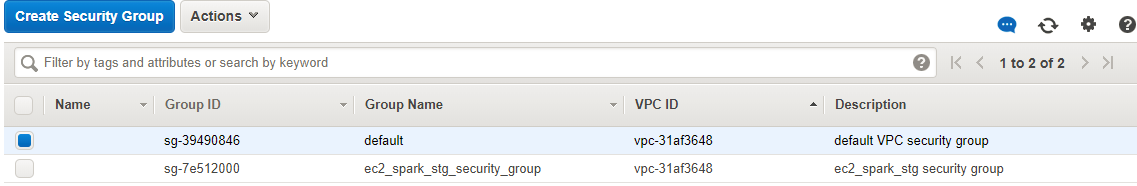
\includegraphics[width=\columnwidth]{images/securitygroup.png}
	\caption{Security group}\label{f:security-group}
\end{figure}

\paragraph{Key Pair:}

Figure~\ref{f:key-pair} shows Key pair created in the deployment.

\begin{figure}[!ht]
	\centering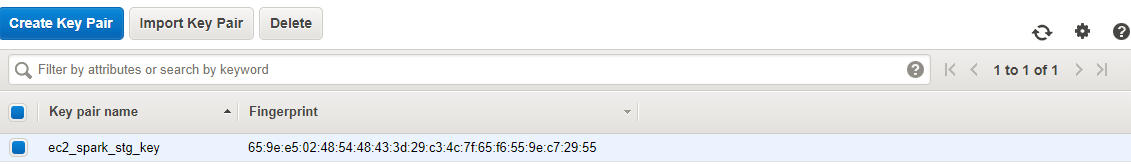
\includegraphics[width=\columnwidth]{images/keypair.png}
	\caption{Key pair}\label{f:key-pair}
\end{figure}

\textbf{EC2~\cite{hid-sp18-511-www-ec2} instances:}

Figure~\ref{f:ec2-instance} shows EC2~\cite{hid-sp18-511-www-ec2}
instances created in the deployment.

\begin{figure}[!ht]
	\centering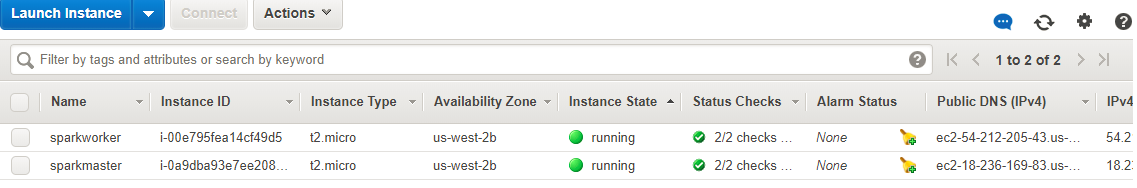
\includegraphics[width=\columnwidth]{images/ec2instances.png}
	\caption{EC2 instance}\label{f:ec2-instance}
\end{figure}


\begin{verbatim}
cd ~/github/cloudmesh-community/$HID.git/project-code
/inventory
\end{verbatim}

Open hosts file and find out the IP address in [sparkmaster] and
[sparkworker] section.

Connect to the Spark worker node using ssh:

\begin{verbatim}
ssh -i ec2_spark_stg_key-private.pem 
ubuntu@<Spark worker IP adddress>
\end{verbatim}

Once you connect to the Spark worker, execute the command:

\begin{verbatim}
sudo start-slave.sh spark://<Spark master IP address>:7077
\end{verbatim}

Validate Spark Apache Cluster up and running by typing the below url
in browser

\begin{verbatim}
http://<Spark master IP address>:8080
\end{verbatim}

Figure~\ref{f:spark-cluster-url} shows Apache
Spark~\cite{hid-sp18-511-www-spark} Cluster URL\@.

\begin{figure}[!ht]
\centering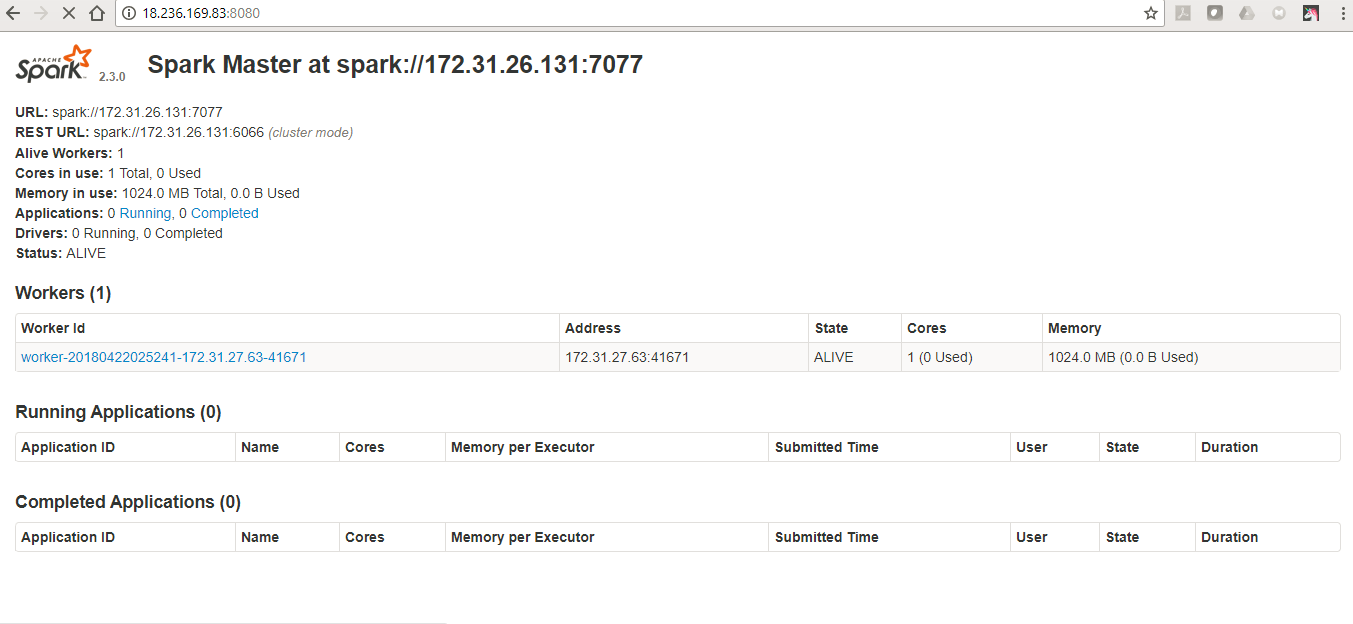
\includegraphics[width=\columnwidth]{images/sparkclusterurl.png}
\caption{Spark Cluster URL}\label{f:spark-cluster-url}
\end{figure}

Connect to Apache Spark~\cite{hid-sp18-511-www-spark} master and
worker and validate Apache Spark shell is functioning properly.  Run
the following command on both master and worker node.

\begin{verbatim}
cd /opt/spark/spark-2.3.0-bin-hadoop2.7/bin
./spark-shell 
\end{verbatim}
 
Figure~\ref{f:spark-shell} shows Apache
Spark~\cite{hid-sp18-511-www-spark} shell command prompt.

\begin{figure}[!ht]
	\centering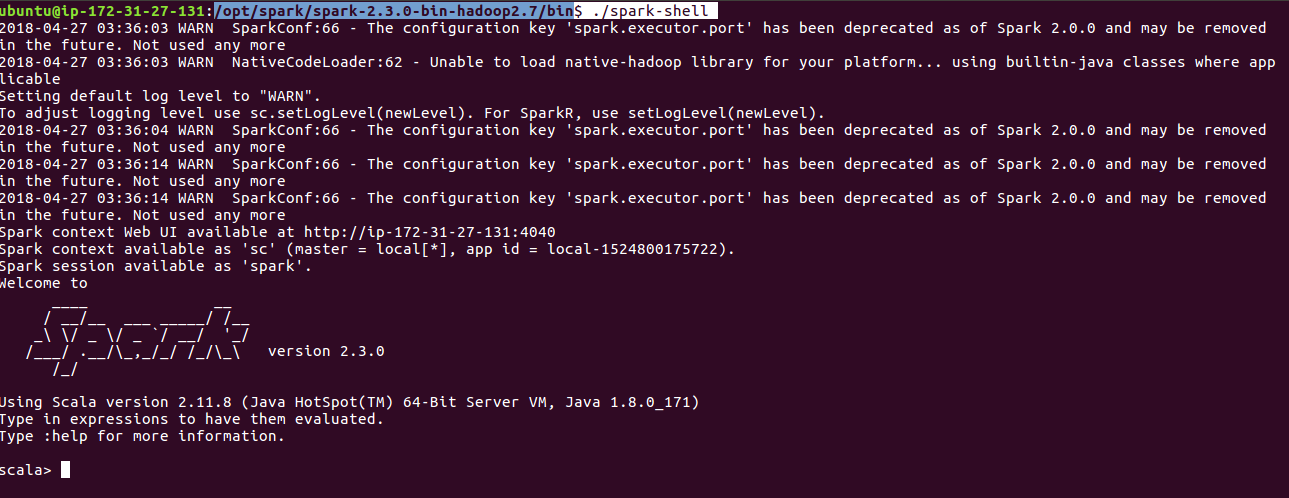
\includegraphics[width=\columnwidth]{images/sparkshell.png}
	\caption{Spark Shell}\label{f:spark-shell}
\end{figure}

\subsection{Data processing on Apache Spark Cluster}

Apache Spark~\cite{hid-sp18-511-www-spark} Cluster can be used for
various data related tasks.  Apache
Spark~\cite{hid-sp18-511-www-spark} can be used for the Batch
processing, Streaming, Machine learning etc. These data processing
related tasks can be written Java, R, Python or Scala.

Apache Spark~\cite{hid-sp18-511-www-spark} distribution come along
with multiple example code. These example code can be used as a
starting point for the hands-on. These example code are available in
Java, R, Python and Scala language.

In this section we will see how data processing related tasks written
in Python language can be submit to Apache
Spark~\cite{hid-sp18-511-www-spark} Cluster. We will use Python
streaming example code in Apache Spark~\cite{hid-sp18-511-www-spark}
distribution to demonstrate the submission of application to Apache
Spark~\cite{hid-sp18-511-www-spark} Cluster.

We will use network word count example for the demonstration. This
example code can be found at the following path in both master and
worker node.

\begin{verbatim}
/opt/spark/spark-2.3.0-bin-hadoop2.7/examples/src/main \
/python/streaming/network_wordcount.py
\end{verbatim}

This program can be executed using the following command.

\begin{verbatim}
cd /opt/spark/spark-2.3.0-bin-hadoop2.7
sudo bin/spark-submit --master spark://172.31.27.119:7077 \
examples/src/main/python/streaming/network_wordcount.py \
localhost 9999
\end{verbatim}

This streaming program require hostname and port number as
argument. This streaming program will connect to the TCP server
specified using the hostname and port number argument to receive the
data.

Execute the program to listen to the TCP server on local host at port
1000 using the following command.

\begin{verbatim}
cd /opt/spark/spark-2.3.0-bin-hadoop2.7
sudo bin/spark-submit --master spark://172.31.27.119:7077 \
examples/src/main/python/streaming/network_wordcount.py \
localhost 9999 
\end{verbatim}

Once the program is executed, it will wait for the data on TCP server
on localhost at port 9999.

We could create a virtual TCP server using the following command.

\begin{verbatim}
sudo nc -lk 9999
\end{verbatim}

The above command will create the TCP server on local host at port
9999. Any data specified in the console will be received by the
streaming program in batches of 1 second interval.

The streaming application will count the number of different words in
each batch and print the initial 10 words on the console.

Figure~\ref{f:python-spark-stream-run-command} shows the command to
run Python stream program and submit to Apache
Spark~\cite{hid-sp18-511-www-spark} Cluster.

\begin{figure}[!ht]
	\centering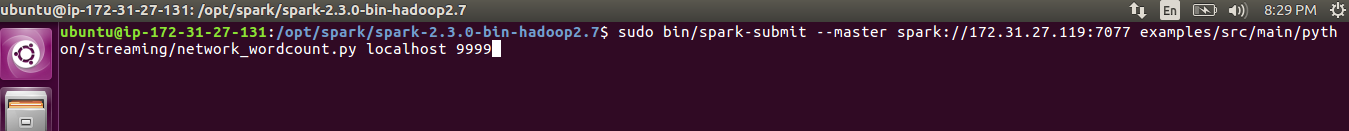
\includegraphics[width=\columnwidth]
        {images/pythonstreamprogruncoammand.png} \caption{Python
	Spark stream run
	command}\label{f:python-spark-stream-run-command}
\end{figure}

Figure~\ref{f:python-stream-tcp-server.png} shows the command to run
TCP server on a particular host and port number. We are running the
TCP server on localhost at port 9999 in this demonstration. We have
ingested few words into the server.

\begin{figure}[!ht]
	\centering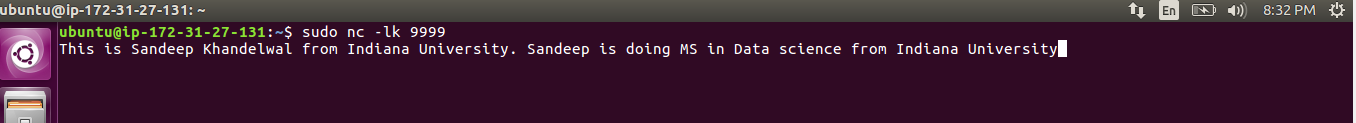
\includegraphics[width=\columnwidth]
        {images/pythonstreamtcpserver.png} \caption{Python
	stream TCP server}\label{f:python-stream-tcp-server.png}
\end{figure}

Figure~\ref{f:python_stream_prog_run_output.png} shows the output of
stream once few of the words are ingested into the TCP server.

\begin{figure}[!ht]
	\centering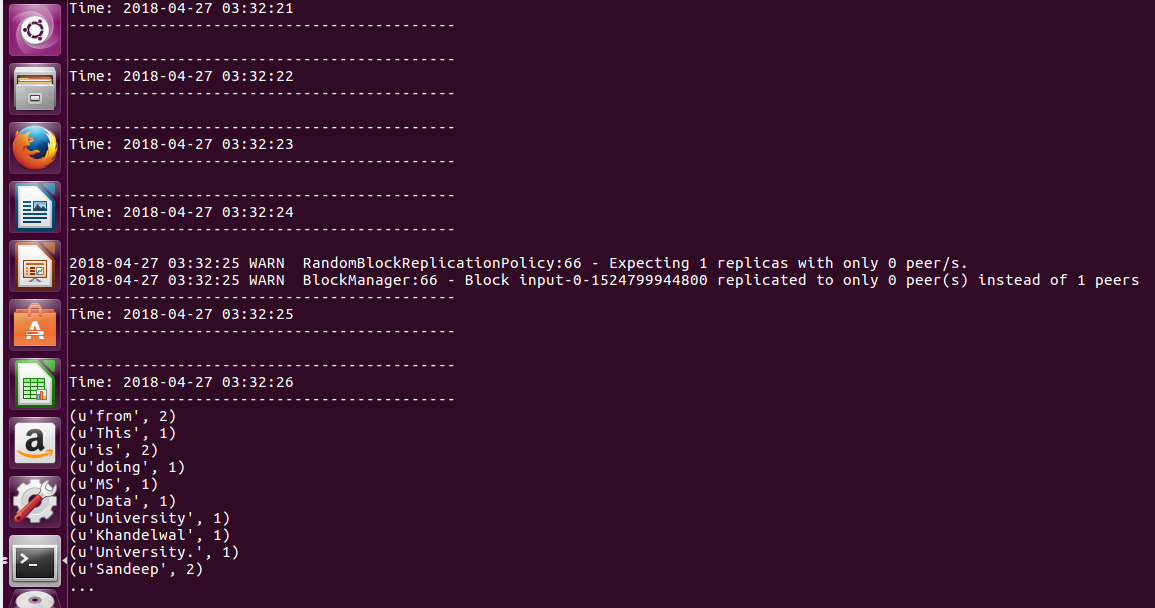
\includegraphics[width=\columnwidth]
        {images/pythonstreamprogrunoutput.png} \caption{Python
	stream output}\label{f:python_stream_prog_run_output.png}
\end{figure}

\subsection{Terminate Apache Spark Cluster}

Execute the following command on the Unix console to terminate Apache
Spark Cluster~\cite{hid-sp18-511-www-spark}.

\begin{verbatim}
cd ~/github/cloudmesh-community/$HID.git/project-code/
ansible-playbook site.yml --tags `terminate'
\end{verbatim}

This command will perform following tasks:

\begin{itemize}
	\item Terminate Apache Spark master node
	\item Terminate Apache Spark worker node
\end{itemize}

Validate Apache Spark~\cite{hid-sp18-511-www-spark} master and Apache
Spark~\cite{hid-sp18-511-www-spark} worker nodes have been terminated
by login to AWS~\cite{hid-sp18-511-www-aws} console.

Figure~\ref{f:ec2-instance-terminate} shows
EC2~\cite{hid-sp18-511-www-ec2} instances terminated.

\begin{figure}[!ht]
	\centering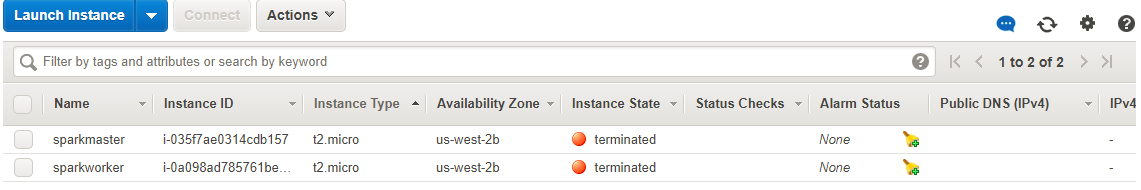
\includegraphics[width=\columnwidth]
        {images/ec2instancesterminate.png} \caption{EC2
	instance termination}\label{f:ec2-instance-terminate}
\end{figure}


\section{Project video}

Two videos to demonstrate the Apache
Spark~\cite{hid-sp18-511-www-spark} automated deployment has been
created and is made available at \cite{??} and \cite{??}. 

The first video shows ....

The sceond video shows ....

This video
walk through all the prerequisites required for the project, demo of
Apache Spark~\cite{hid-sp18-511-www-spark} deployment and termination.

\TODO{NO URLS IN THE PAPER. use citations}
\begin{itemize}
	\item
        \href{https://d1b10bmlvqabco.cloudfront.net/attach/%
        jbkvbp3ed3m2ez/j6r57sr2IDo/jgenhk1lk5ly/%
        hidsp18511\_AWS\_EC2\_Deployment\_1.mp4}
        {Apache Spark deployment demo part 1}
        \item
        \href{https://d1b10bmlvqabco.cloudfront.net/attach/%
        jbkvbp3ed3m2ez/j6r57sr2IDo/jgeniacbvn7m/%
        hidsp18511\_AWS\_EC2\_Deployment\_2.mp4}
        {Apache	Spark deployment demo part 2}
\end{itemize}

\section{Results}

Table~\ref{t:results-table} provides the benchmark results.

\TODO{TEXT MISSING}

\begin{table}[htb]
	\centering
	\caption{Results}\label{t:results-table}
	\begin{tabular}{ll} 
		\textbf{Setup} & \textbf{Duration (in minutes)} \\ 
		Apache Spark Cluster deployment  & 21 mins \\
		Apache Spark Cluster termination & 1 min \\
	\end{tabular}
\end{table}


\section{Conclusion}

We are successfully able to deploy Apache
Spark~\cite{hid-sp18-511-www-spark} Cluster on
AWS~\cite{hid-sp18-511-www-aws} EC2~\cite{hid-sp18-511-www-ec2}
instances using Ansible~\cite{hid-sp18-511-www-ansible} deployment and
configuration tool on a single click. The amount of duration for end
to end deployment was only few minutes instead of hours/days which was
the case in earlier days when Cloud was not there. We were able to do
streaming using deployed Apache Spark~\cite{hid-sp18-511-www-spark}
Cluster. This could be used for any kind of data processing need. We
were also able to terminate the instances on a single click only in 1
minute.

This project could be further enhanced to add other
AWS~\cite{hid-sp18-511-www-aws} EC2~\cite{hid-sp18-511-www-ec2}
services. We could create service for virtual network, storage etc as
per requirement.

\begin{acks}

  The authors would like to thank Dr.~Gregor~von~Laszewski for his
  support and suggestions to write this paper.

\end{acks}

\bibliographystyle{ACM-Reference-Format}
\bibliography{report} 

